\documentclass[aspectratio=149,12pt]{beamer}
%依赖包
\usepackage{amsmath,amssymb,enumerate,epsfig,bbm,calc,color,ifthen,capt-of,multimedia,hyperref}
\usepackage{ctex}
\CTEXoptions[today=old]
\usepackage{multicol}
\usepackage{hyperref} 
\usepackage{cite}
\usepackage{booktabs}
\usepackage{graphicx}
%自定义颜色
\definecolor{szeged}{RGB}{153,153,217}%主题色
\definecolor{sme}{RGB}{41,22,111} %深港微配色
\definecolor{sust-orange}{RGB}{237,108,0}
\definecolor{sust-green}{RGB}{0,63,67}
\definecolor{sust-blue}{RGB}{43,183,179}
\setbeamercolor{bluewhite}{bg=sme!80,fg=white}
\setbeamercolor{whiteblue}{bg=white,fg=sme!80}
\setbeamercolor{orangeblue}{bg=sust-orange!80,fg=sme}
\setbeamercolor{whiteblute}{bg=white,fg=sme!80}
%设置主题
\usepackage{SME-theme}%使用深港微蓝色主题
%\usepackage{SUSTech-theme}%使用南科大橙色主题
%取消导航bar
%\setbeamertemplate{navigation symbols}{} 
% 设置目录
\AtBeginSection[]
{
	\begin{frame}<beamer>
	\frametitle{Outline}
	\tableofcontents[currentsection]
	\end{frame}
}
\beamerdefaultoverlayspecification{<+->}


% ---------------------------------------------------------------
\title{This is the sample of PPT}
\subtitle{This is the subtitle of PPT}
\author{Sakuranetin}
\institute{Southern University of Science and Technology}
\date{\today}

%鸣谢:https://github.com/SUSTC/sustech-slides 提供结构参考
%			B站up:joefsong提供疑难解惑
\begin{document}
% ---------------------------------------------------------------

\frame{\titlepage}

\begin{frame}{Outline}
\tableofcontents
\end{frame}
% ---------------------------------------------------------------

\section{Abstract}
\begin{frame}{Abstract}

\end{frame}


\section{Introduction}
\begin{frame}{Introduction}
	\begin{columns}[T] % align columns
		\begin{column}<0->{.48\textwidth}
		\begin{figure}[thpb]
			\centering
			\resizebox{1\linewidth}{!}{
				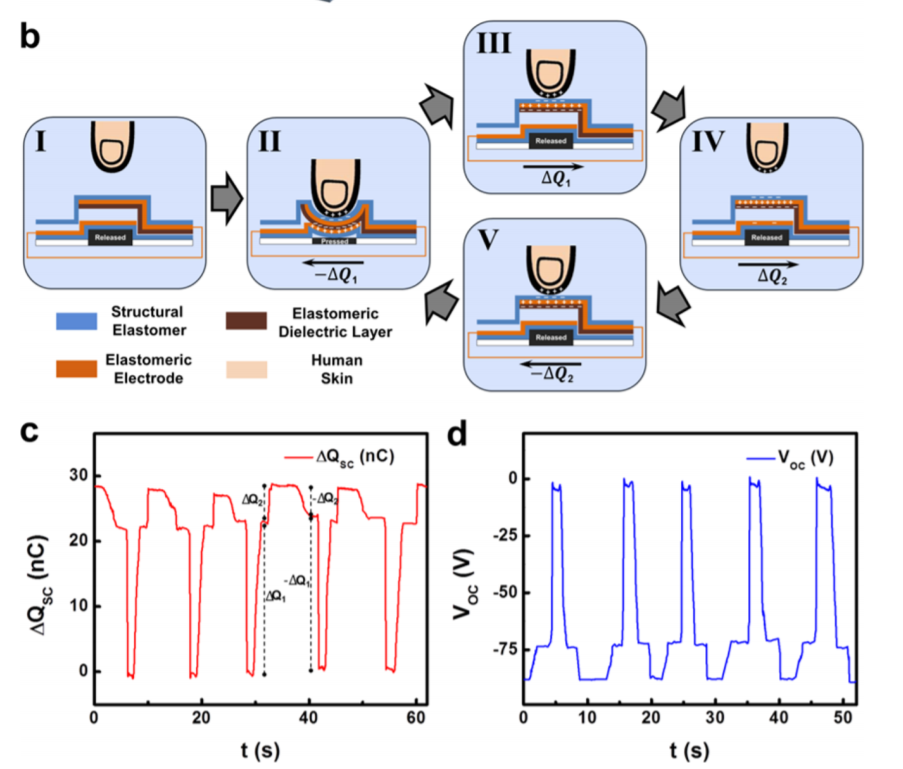
\includegraphics{figures/02.png}
			}
			\label{fig:Introduction}
		\end{figure}
		\end{column}%
	%\hfill%
		\begin{column}<0->{.48\paperwidth}
		\begin{itemize}
			\item Solely
			fabricated by elastomeric silicone materials, the TENG renders
			high \alert{flexibility} and \alert{stretchability}.
			\item Benefiting from flexible
			and stretchable layers for contact electrification, the \alert{tribocharge density} could be significantly improved because of more adequate contact.
		\end{itemize}
		\end{column}%
	\end{columns}
\end{frame}
% ---------------------------------------------------------------


% ---------------------------------------------------------------
\section{Results and discussions}
\subsection{Structure and materials}
\begin{frame}
\begin{figure}[thpb]
\centering

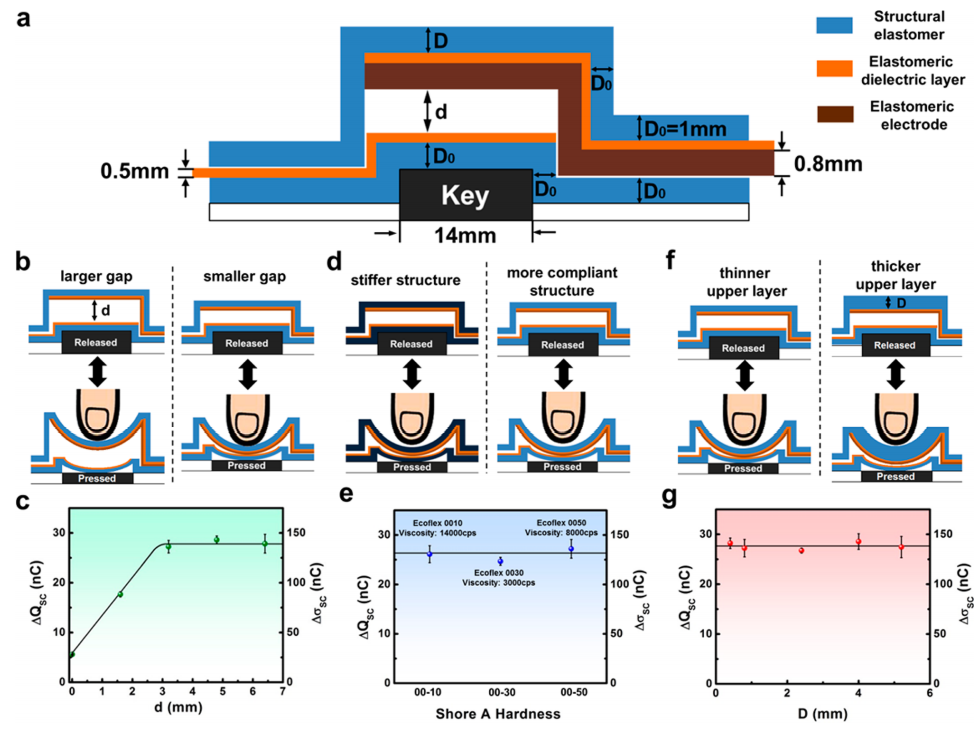
\includegraphics[scale=0.26]{figures/03.png}

\end{figure}
\end{frame}

\subsection{Frequency and forces}
\begin{frame}

\end{frame}


% ---------------------------------------------------------------
\section{Conclusions}
\begin{frame}{Conclusions}
\begin{itemize}
\item  Demonstrated a highly flexible TENG solely fabricated using elastomeric materials for harvesting biomechanical energy from a \alert{keyboard} and \alert{buttons}.
\item $\cdots$
\end{itemize}
\end{frame}

\begin{frame}
\Huge\qquad Thank you for listening!
\end{frame}
% ---------------------------------------------------------------
\end{document}